\documentclass[onecolumn]{article}
% \documentclass[twocolumn]{article}

\usepackage{style/arxiv}
% \usepackage{style/roundenv}

% --- Packages ---
\usepackage[utf8]{inputenc} % 允许使用 UTF-8 编码输入(pdflatex 下常用;xelatex/lualatex 不需要)
\usepackage[T1]{fontenc}    % 使用 T1 字体编码(更好地支持西欧字符、断词和复制粘贴)

\usepackage{amsmath, amssymb, amsthm}

\usepackage{hyperref}       % 生成可点击的超链接(目录、引用、网址等),并支持 \autoref
\usepackage{cleveref}       % 智能引用命令 \cref/\Cref,自动加上“图/表/公式”等前缀,可本地化
\usepackage{url}            % 提供更简单的 URL 格式化(在 hyperref 未加载时也能用)

\usepackage{booktabs}       % 提供专业级表格命令(\toprule, \midrule, \bottomrule)
\usepackage{amsfonts}       % 数学字体扩展(黑板粗体等,ℝ, ℤ, ℕ)
\usepackage{nicefrac}       % 紧凑的分数形式(例如 ½, ¾,用 \nicefrac{1}{2})
\usepackage{microtype}      % 微排版优化(字符间距、断字,更美观)

\usepackage{lipsum}         % 生成示例文字(Lorem ipsum),常用于排版测试
\usepackage{graphicx}       % 插图支持(\includegraphics)

\usepackage{natbib}         % 高级参考文献管理(支持 \citet, \citep 等命令)
\usepackage{doi}            % 在参考文献中格式化 DOI,自动生成可点击链接

\usepackage{pgffor}         % 提供 \foreach 循环功能(来自 TikZ/PGF,可批量生成子图、表格等)
\usepackage{subcaption}     % 提供 subfigure 环境,用于排版子图并添加独立标题
\usepackage{wrapfig}        % 提供 wrapfigure / wraptable 环境,使图表可以与正文文字环绕排版
\usepackage{enumitem}       % 增强 itemize/enumerate 列表,支持自定义编号、缩进、间距等

\usepackage[ruled,vlined]{algorithm2e}  % 独立的算法宏包,提供 algorithm 环境和伪代码命令
\crefname{algocf}{algorithm}{algorithms}
\Crefname{algocf}{Algorithm}{Algorithms}

% --- Theorem-like environments ---
\newtheorem{theorem}{Theorem}[section]
\newtheorem{lemma}[theorem]{Lemma}
\newtheorem{corollary}[theorem]{Corollary}
\newtheorem{proposition}[theorem]{Proposition}

\theoremstyle{definition}
\newtheorem{definition}[theorem]{Definition}
\newtheorem{condition}[theorem]{Condition}
\newtheorem{example}[theorem]{Example}

\theoremstyle{remark}
\newtheorem*{remark}{Remark}
\newtheorem*{note}{Note}

% --- main ---
\title{A template for the \emph{arxiv} style}

% 作者行:不用可选参数
\author{%
  Chong Zhou\affmark{\footlabel{1}1,2},
  Chen Change Loy\affmark{1},
  Bo Dai\affmark{2}
}

% 机构行(复用数字角标)
\affiliations{%
  \affmark{1} S-Lab, Nanyang Technological University\\
  \affmark{2} Shanghai AI Laboratory
}

% 邮箱集中一行
\emailline{%
  \{chong033, ccloy\}@ntu.edu.sg \quad daibo@pjlab.org.cn
}

% 角标显示在页脚
\footline{
  \foottext{1}{Equal contribution}
}


%%% Add PDF metadata to help others organize their library
%%% Once the PDF is generated, you can check the metadata with
%%% $ pdfinfo template.pdf
\hypersetup{
pdftitle={A template for the arxiv style},
pdfsubject={q-bio.NC, q-bio.QM},
pdfauthor={David S.~Hippocampus, Elias D.~Striatum},
pdfkeywords={First keyword, Second keyword, More},
}

\begin{document}
\maketitle

\begin{abstract}
	\lipsum[1]
\end{abstract}


% keywords can be removed
% \keywords{First keyword \and Second keyword \and More}


\section{Headings: first level}

\lipsum[2]

\subsection{Headings: second level}
\lipsum[3]

\subsubsection{Headings: third level}
\lipsum[4]

\paragraph{Paragraph}
\lipsum[5]



\section{Examples of basic functions}
\label{sec:others}

\verb+\autoref+: See \autoref{sec:others}. \\
\verb+\cref+: See \cref{sec:others}. 

\subsection{Equation}

\verb+\autoref+: See \autoref{eq:eq}. \\
\verb+\cref+: See \cref{eq:eq}. 

\begin{equation}
{\frac {\alpha _{i}(t)a^{w_t}_{ij}\beta _{j}(t+1)b^{v_{t+1}}_{j}(y_{t+1})}{\sum _{i=1}^{N} \sum _{j=1}^{N} \alpha _{i}(t)a^{w_t}_{ij}\beta _{j}(t+1)b^{v_{t+1}}_{j}(y_{t+1})}}
    \label{eq:eq}
\end{equation}

\subsection{Citations}

Here is an example usage of the two main commands (\verb+citet+ and \verb+citep+): Some people thought a thing \citep{kour2014real, hadash2018estimate} but other people thought something else \citep{kour2014fast}. Many people have speculated that if we knew exactly why \citet{kour2014fast} thought this\dots

\subsection{Footnote}

Here is how you add footnotes. \footnote{Sample of the first footnote.}

\subsection{Figures}

\verb+\autoref+: See \autoref{fig:fig1} and \autoref{fig:subfig1}. \\
\verb+\cref+: See \cref{fig:fig1} and \cref{fig:subfig1}. 


\begin{figure}[h]
    \centering
    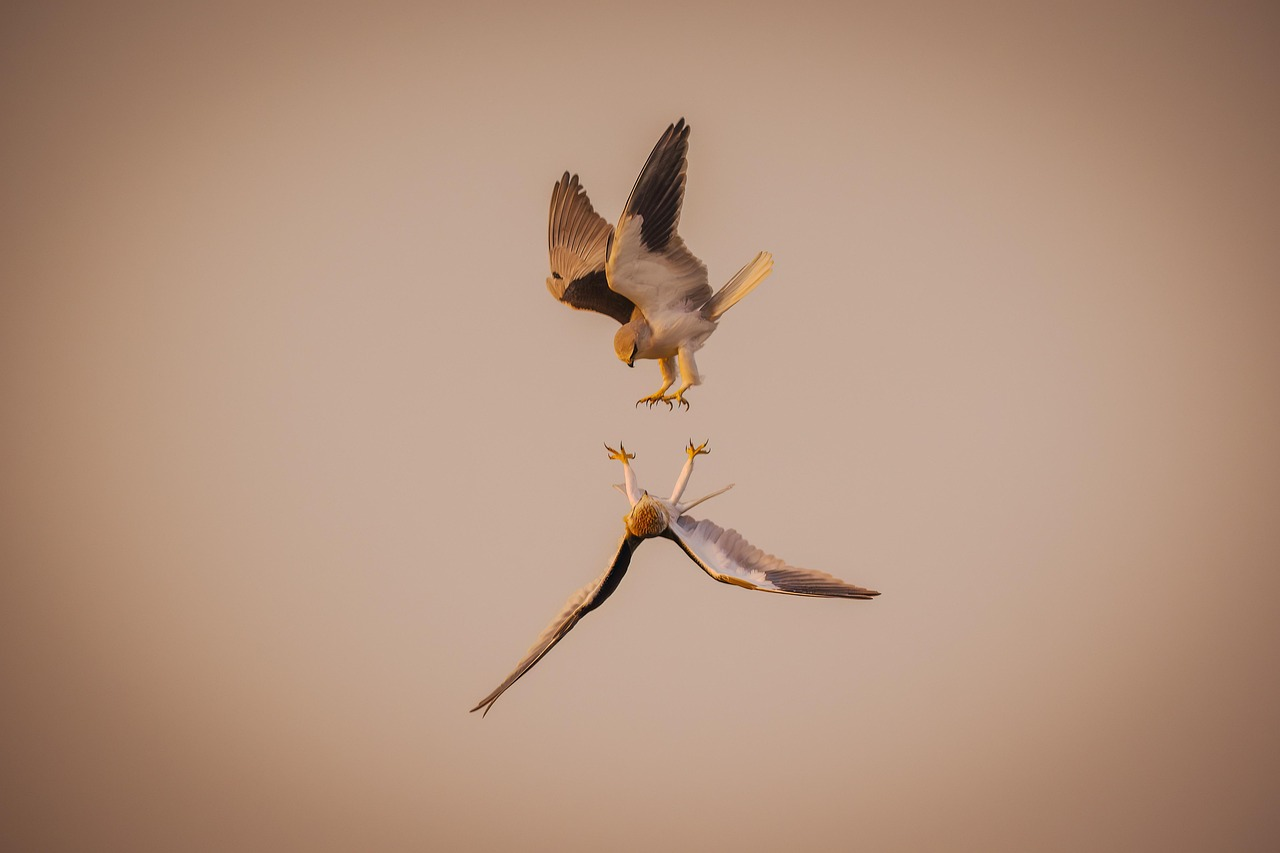
\includegraphics[width=.3\linewidth]{fig/example1.jpg}
    \caption{Sample figure caption}
    \label{fig:fig1}
\end{figure}

\begin{figure}[h]
    \centering
    \foreach \i [evaluate=\i as \n using int(\i+1)] in {0,...,3} {
        \begin{subfigure}[b]{0.20\textwidth}
            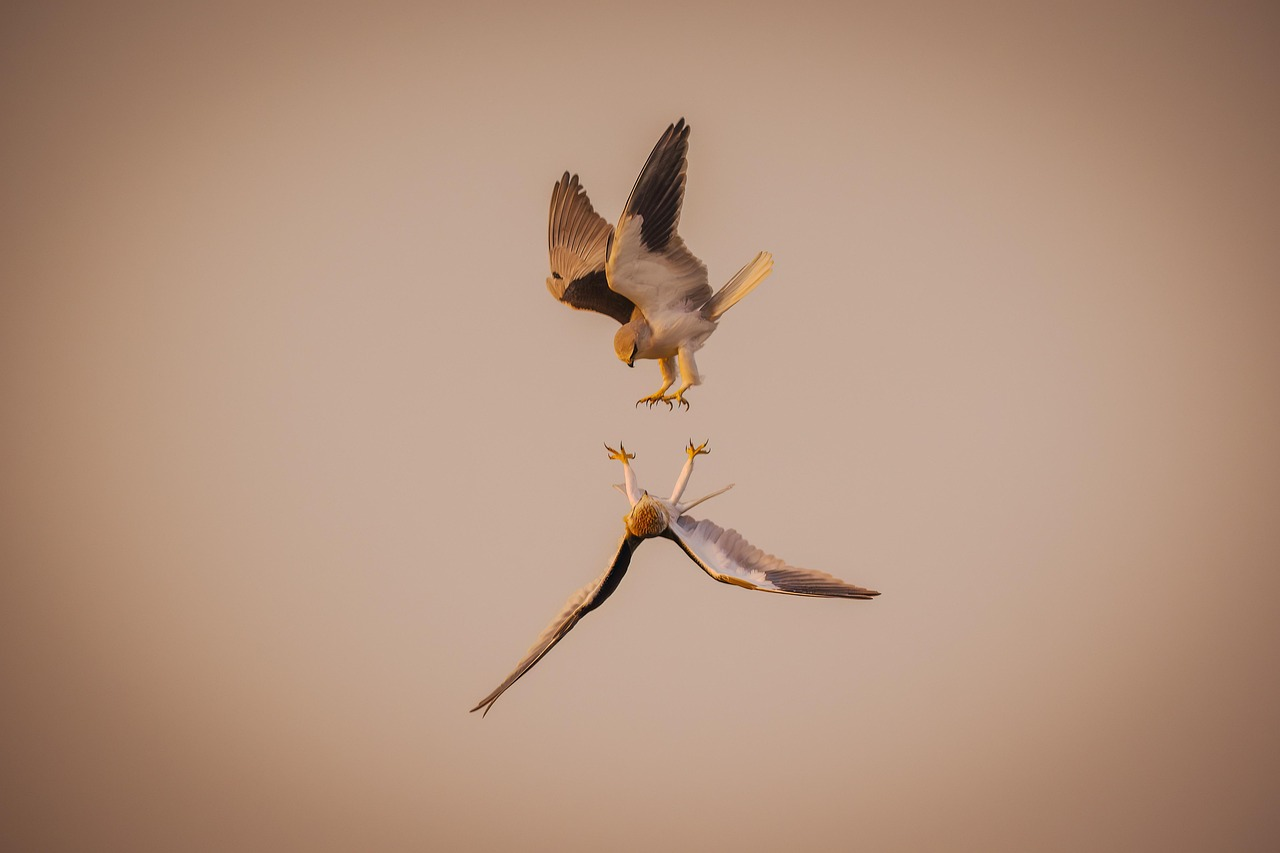
\includegraphics[width=\linewidth]{fig/example1.jpg}
            \caption{Subfigure Caption}
            \label{fig:subfig\n}
        \end{subfigure}
    }\\[0.5em] 
    \foreach \i in {0,...,3} {
        \begin{subfigure}[b]{0.20\textwidth}
            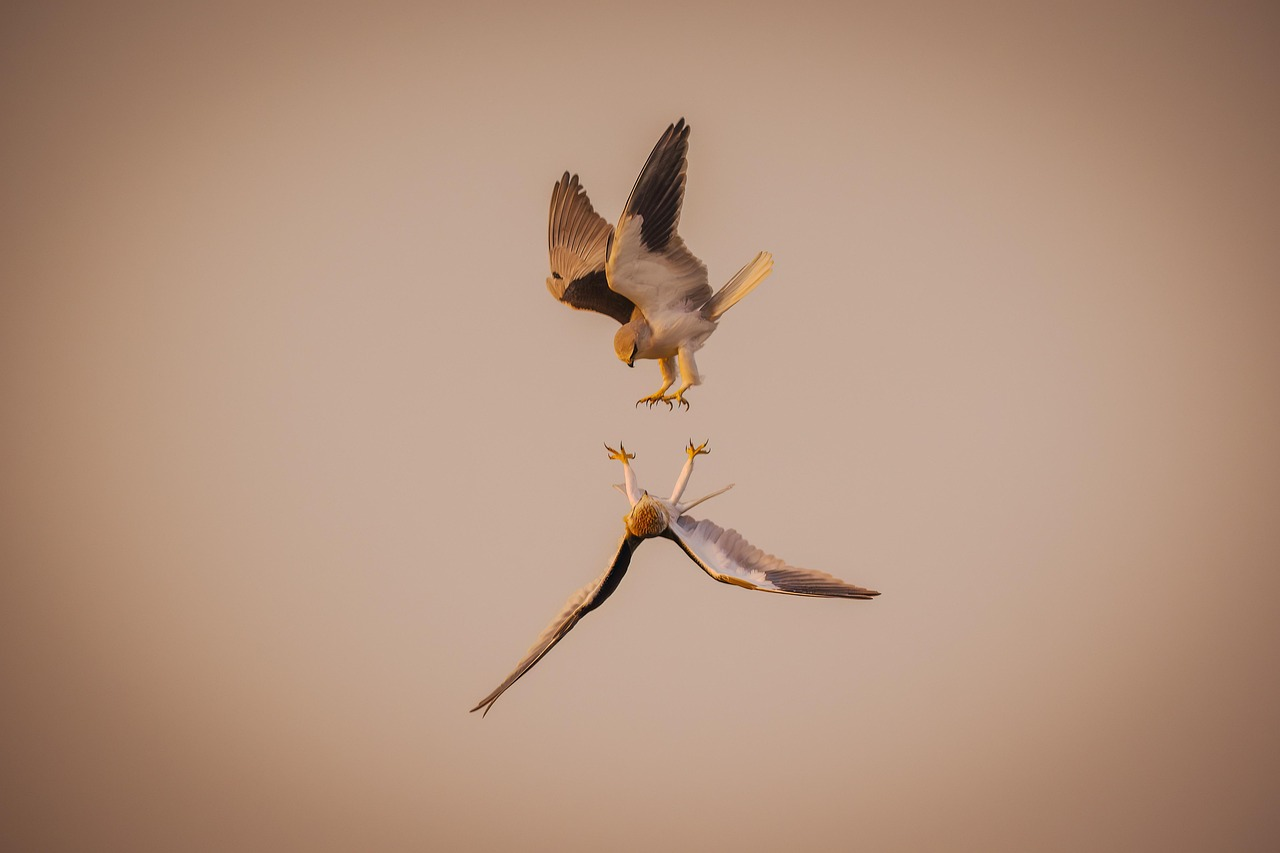
\includegraphics[width=\linewidth]{fig/example1.jpg}
            \caption{Subfigure Caption}
        \end{subfigure}
    }\\
    \caption{Multiple image placement caption}
    \label{fig:appendix_gradual-cifar-10-c}
\end{figure}

\lipsum[6]

\begin{wrapfigure}{r}{0.35\linewidth}
    \centering
    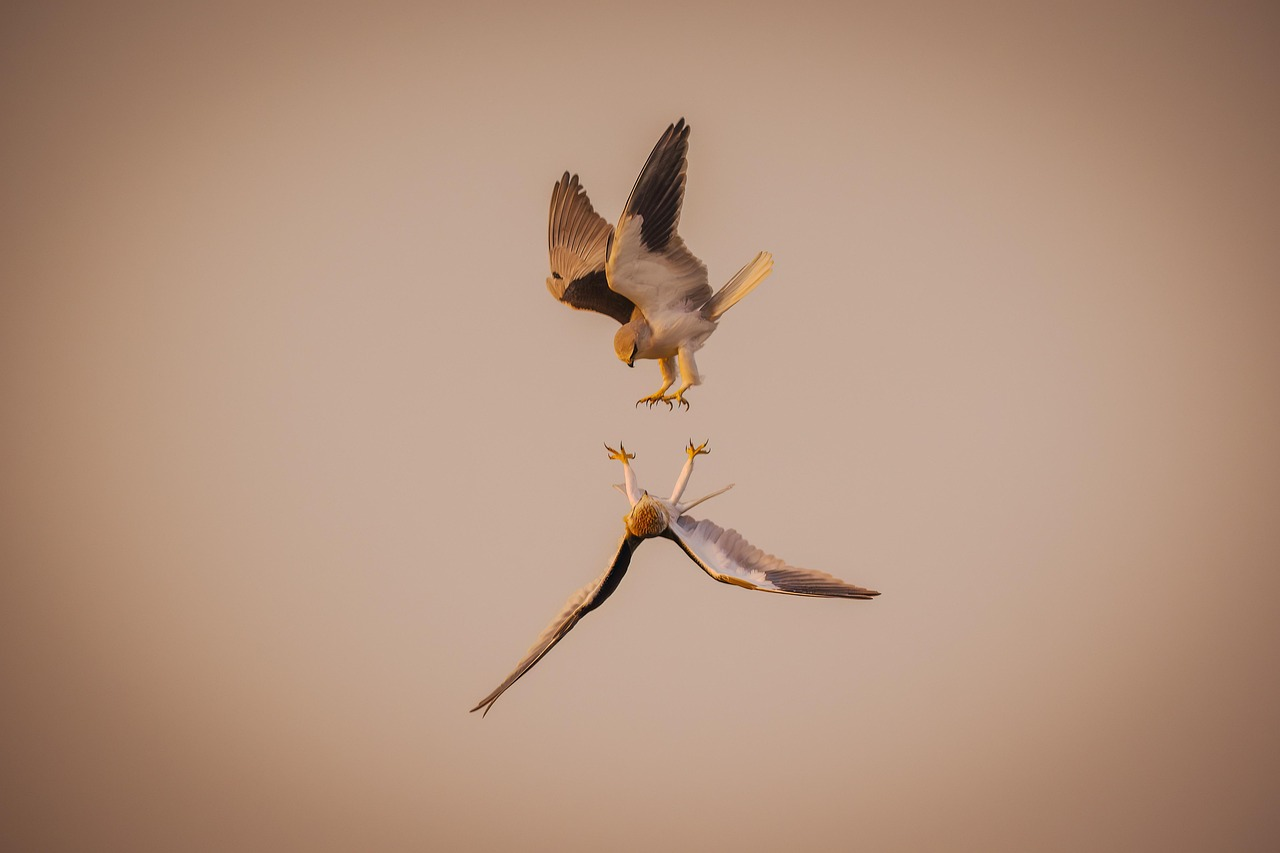
\includegraphics[width=.9\linewidth]{fig/example1.jpg}
    \caption{Sample figure caption}
\end{wrapfigure}

\lipsum[7-8]

\subsection{Tables}

\verb+\autoref+: See \autoref{tab:table}. \\
\verb+\cref+:  See \cref{tab:table}. 

\begin{table}[h]
    \caption{Sample table title}
    \centering
    \begin{tabular}{lll}
        \toprule
        \multicolumn{2}{c}{Part}                   \\
        \cmidrule(r){1-2}
        Name     & Description     & Size ($\mu$m) \\
        \midrule
        Dendrite & Input terminal  & $\sim$100     \\
        Axon     & Output terminal & $\sim$10      \\
        Soma     & Cell body       & up to $10^6$  \\
        \bottomrule
    \end{tabular}
    \label{tab:table}
\end{table}

\begin{wraptable}{r}{5cm}
    \centering
    % \vspace{-1.0cm}
    \caption{Sample table title}
    \resizebox{5cm}{!}{%
        \begin{tabular}{c p{5.0cm}}
        \toprule
        \textbf{Symbol} & \textbf{Meaning} \\
        \midrule
        $\mathcal{D}_i$ & Distribution of domain $i$ ($i{=}0{:}n$)  \\
        $\mathcal{Z}_i$ & Feature distribution induced by $\mathcal{D}_i$ \\
        $r(\cdot;\phi)$ & Feature extractor, $\mathbb{X} \rightarrow \mathbb{Z}$ \\
        $k(\cdot;\varphi)$ & Label head (classifier), $\mathbb{Z} \rightarrow \mathbb{Y}$. \\
        $f(\cdot;\theta)$ & Witness network; $g=f_T-f_0$.\\
        \bottomrule
        \end{tabular}
    }
\end{wraptable}

\lipsum[8-9]

\subsection{Lists}

\verb+\autoref+: See \autoref{itm:first}. \\
\verb+\cref+: See \cref{itm:first}.

\begin{itemize}
    \item Lorem ipsum dolor sit amet
    \item consectetur adipiscing elit.
    \item Aliquam dignissim blandit est, in dictum tortor gravida eget. In ac rutrum magna.
\end{itemize}

\begin{enumerate}[label=\Roman*.]
    \item \label{itm:first} Lorem ipsum dolor sit amet
    \item consectetur adipiscing elit.
    \item Aliquam dignissim blandit est, in dictum tortor gravida eget. In ac rutrum magna.
\end{enumerate}

\subsection{Algorithm}

\verb+\autoref+: See \autoref{alg:flow}. \\
\verb+\cref+: See \cref{alg:flow}.

\begin{algorithm}[h]
\caption{Euclid’s Algorithm for GCD}   % 算法标题
\KwIn{$a, b$}                          % 输入
\KwOut{$\gcd(a,b)$}                    % 输出

\While{$b \neq 0$}{                    % While 循环
    $r \gets a \bmod b$\;              % 语句,每行结尾用分号 \;
    $a \gets b$\;
    $b \gets r$\;
}
\Return $a$\;                          % 返回结果
\label{alg:flow}
\end{algorithm}

\section{Examples of Theorem Environments}

\verb+\autoref+: We can see \autoref{thm:pythagoras}, \autoref{lem:square}, \autoref{cor:nonnegative}, 
\autoref{prop:primes}, \autoref{def:metric}, \autoref{cond:stability}, 
\autoref{ex:stability}, \autoref{rem:control}, and \autoref{note:pythagoras}. \\
\verb+\cref+: We can see \cref{thm:pythagoras}, \cref{lem:square}, \cref{cor:nonnegative}, 
\cref{prop:primes}, \cref{def:metric}, \cref{cond:stability}, 
\cref{ex:stability}, \cref{rem:control}, and \cref{note:pythagoras}.

\begin{theorem}[Pythagoras] % 定理
\label{thm:pythagoras}
If a triangle is right-angled, then the square of the hypotenuse equals the sum of the squares of the other two sides.
\end{theorem}

\begin{lemma} % 引理
\label{lem:square}
For any real numbers $a$ and $b$, we have $(a+b)^2 \geq 0$.
\end{lemma}

\begin{corollary} % 推论
\label{cor:nonnegative}
Every real number has a non-negative square.
\end{corollary}

\begin{proposition} % 命题
\label{prop:primes}
The set of prime numbers is infinite.
\end{proposition}

\begin{definition}[Metric Space] % 定义
\label{def:metric}
A \emph{metric space} is a pair $(X,d)$ where $X$ is a set and $d:X\times X\to\mathbb{R}$ satisfies positivity, symmetry, and the triangle inequality.
\end{definition}

\begin{condition}[Stability] % 条件
\label{cond:stability}
If $|f(x)| \leq \alpha|x|$ with $0<\alpha<1$, then the system is stable.
\end{condition}

\begin{example} % 例子
\label{ex:stability}
Let $f(x)=\tfrac{1}{2}x$. Then the condition of stability is satisfied.
\end{example}

\begin{remark} % 注释
\label{rem:control}
Conditions are often used in optimization and control theory.
\end{remark}

\begin{note} % 附注
\label{note:pythagoras}
The proof of Pythagoras can be done geometrically or algebraically.
\end{note}

\begin{proof} % 证明
It follows directly from the axioms of $d$. 
\end{proof}



%%%%%%%%%%%%%%%%%%%%%%%%%%%%%%%%%%%%%%%%%%%%%%%%%%%%%%

\bibliographystyle{unsrtnat}
\bibliography{references}  %%% Uncomment this line and comment out the ``thebibliography'' section below to use the external .bib file (using bibtex) .


%%% Uncomment this section and comment out the \bibliography{references} line above to use inline references.
% \begin{thebibliography}{1}

% 	\bibitem{kour2014real}
% 	George Kour and Raid Saabne.
% 	\newblock Real-time segmentation of on-line handwritten arabic script.
% 	\newblock In {\em Frontiers in Handwriting Recognition (ICFHR), 2014 14th
% 			International Conference on}, pages 417--422. IEEE, 2014.

% 	\bibitem{kour2014fast}
% 	George Kour and Raid Saabne.
% 	\newblock Fast classification of handwritten on-line arabic characters.
% 	\newblock In {\em Soft Computing and Pattern Recognition (SoCPaR), 2014 6th
% 			International Conference of}, pages 312--318. IEEE, 2014.

% 	\bibitem{hadash2018estimate}
% 	Guy Hadash, Einat Kermany, Boaz Carmeli, Ofer Lavi, George Kour, and Alon
% 	Jacovi.
% 	\newblock Estimate and replace: A novel approach to integrating deep neural
% 	networks with existing applications.
% 	\newblock {\em arXiv preprint arXiv:1804.09028}, 2018.

% \end{thebibliography}

% WARNING: do not forget to delete the supplementary pages from your submission 
\appendix
\onecolumn
% \setcounter{page}{1}
\maketitlesupplementary

\section{Rationale}
\label{sec:rationale}

\verb+\autoref+: See \autoref{sec:rationale}. \\
\verb+\cref+: See \cref{sec:rationale}.

\lipsum[10]

\end{document}
